\section{Overview}

We first provide an overview of our approach.
The structure of the code transformation tool is 
illustrated in figure \ref{sysarch}.
The tool is composed of five modules: Python code parser,
class hierarchy analyzer, API pattern analyzer, AST transformer,
and code generator.

\begin{figure}[ht!]
  \centering
  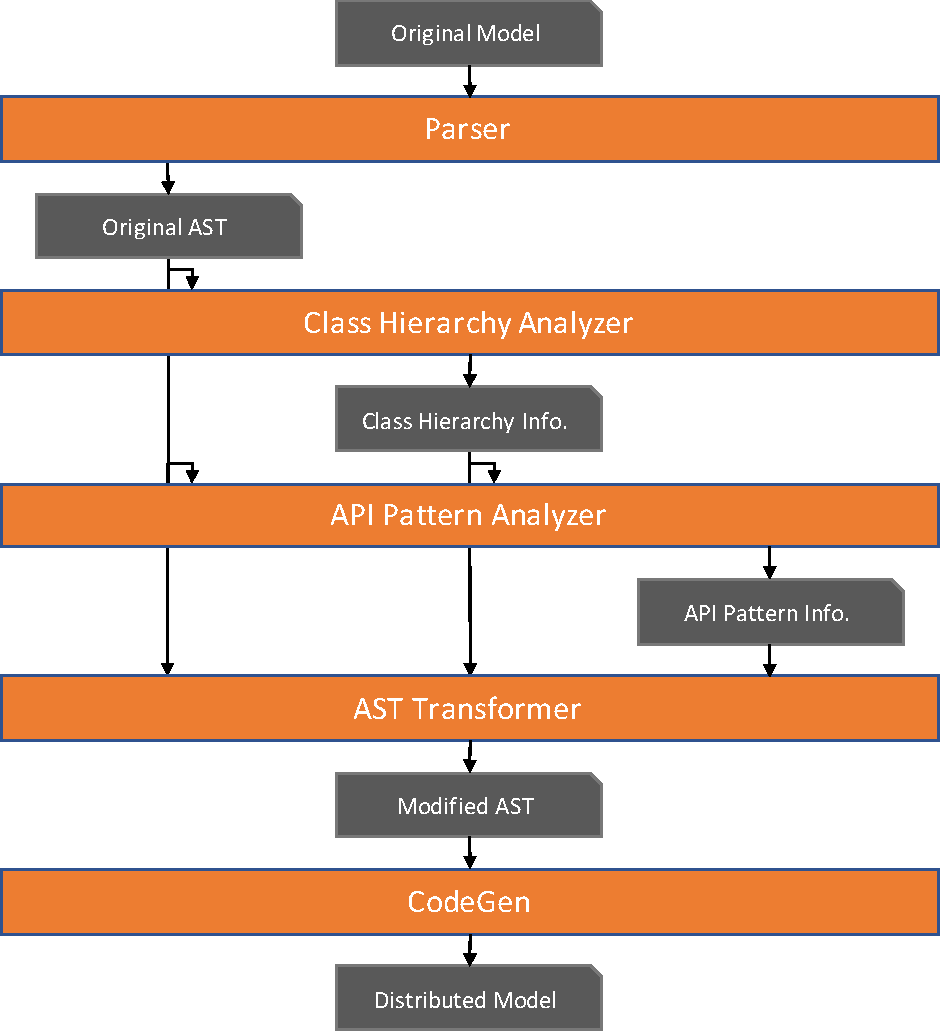
\includegraphics[width=0.5\textwidth]{tool-arch.pdf}
  \caption{The code transformation tool module design diagram}
  \label{sysarch}
\end{figure}

To correctly transform TensorFlow DL models,
it is important to apply appropriate transformation rules
for different type of training codes.
We identified that class inheritance information and
the patterns of traning API usage is essential to 
select the correct transformation rule. 
In this end, our approach analyzes \textit{class hierarchy}
and \textit{training API pattern} in the input training code.
The transformer receives the input training code AST and
additionally class hierarchy and API pattern information
to select the correct set of transformation rules among the candidates
and apply it to the input code AST.

\textbf{Parser}
Parser is the module that parses input Python code package
into the set of ASTs.
We assume that the input single-GPU-based model is given as a Python code
package that resides in a single file directory.
Given the directory, the parser module first parses all Python code files
in the package to ASTs.
The Python abstract syntax and details on the parser implementation
are described in section \ref{sec:pysyn}.

Before the ASTs are transformed, the software performs two analyses, 
which are \textit{class hierarchy analysis} and 
\textit{API pattern analysis}.
These analyses provide necessary information to identify the
location and kind of the transformation target codes in the model
and select the correct transformation rule for the given input model.

\textbf{Class Hierarchy Analyzer}
Class hierarchy analyzer module analyzes the class inheritance relation
between user-defined classes and TensorFlow library classes and
outputs the class hierarchy graph.
During the API pattern analysis and AST transformation phase,
the software need to identify subclass relationship between
classes appearing in the code.
To support this, we implemented the class hierarchy analysis
for Python codes as the class hierarchy analyzer module.
The class hierarchy analyzer module produces the class hierarchy graph
for the model package and returns it to the API pattern analyzer and 
AST transformer modules. The details of the class hierarchy analyzer are
described in section \ref{sec:cha}.

\textbf{Training API Pattern Analyzer}
Training API pattern analyzer module 
indentifies the TensorFlow training APIs used in the training code AST
and returns the training API pattern for the code. (TODO: clarify?)
TensorFlow provides multiple APIs to define and invoke the training process.
To correctly transform a single-GPU-based model training code into
the distributed code, the transformation software must identify
training APIs used in the code and select the appropriate transformation rule.
The training API pattern analyzer matches the \textit{training API pattern}
against the input training codes to categorize them and select
the correct transformation rule. The details of the training API pattern
analyzer are described in section \ref{sec:pattern}.

\textbf{AST Transformer}
AST transformer module applies the correct transformation to the
training code AST to retain the distributed training code AST.
Here, the "correct" transformation is the set of transformation rules
appropriate for the given class hierarchy information and
training API pattern of the input training code.
We defined formal transformation rules which are composed of
\textit{transform functions} from ASTs to ASTs.
By applying the transform function to the input AST,
the AST transformer module outputs the transformed AST as an output.
The details of the AST transformer is described in section \ref{sec:trans}
